\chapter{複合玻色子、自旋表示與狄拉克倍增}

\section{交換對稱性與複合玻色子}

開篇提出的是一個關於複合粒子的真正悖論：如果兩個費米子組成一個玻色子，那麼兩個這樣的玻色子能否佔據同一個狀態，而不違反費米子排他原理？答案得從交換規則本身說起。

假設以含有兩個自變數的波函數描述兩個全同粒子。符號\(x\)和\(y\)標記兩個粒子的位置；它們並不代表兩種不同的粒子。玻色子的波函數是對稱的，費米子的波函數則是反對稱的：
\begin{equation}
\Psi_B(x,y)=\Psi_B(y,x),
\qquad
\Psi_F(x,y)=-\Psi_F(y,x).
\end{equation}
這種對稱性表示，交換兩個不可區分的粒子不會產生新的物理狀態。

兩個玻色子當然可以佔據同一個單粒子態。若該態的波函數為\(\varphi\)，兩粒子態的乘積就是
\begin{equation}
\Psi(x,y)=\varphi(x)\varphi(y).
\end{equation}
波函數是普通的複值函數，不是算符或矩陣，因此函數值可以交換順序：
\begin{equation}
\varphi(x)\varphi(y)=\varphi(y)\varphi(x).
\end{equation}
所以這個乘積是對稱的。同樣的構造無法得到非零的兩費米子態，因為反對稱性會要求
\begin{equation}
\varphi(x)\varphi(y)=-\varphi(y)\varphi(x),
\end{equation}
但不帶負號的兩邊其實相等。

更一般地，從任意兩粒子波函數\(F(x,y)\)出發，不預設它具有任何交換對稱性。忽略歸一化後，它的對稱部分和反對稱部分為
\begin{align}
F_{\mathrm{sym}}(x,y)&=F(x,y)+F(y,x),\\
F_{\mathrm{asym}}(x,y)&=F(x,y)-F(y,x).
\end{align}
直接交換自變數即可驗證：
\begin{align}
F_{\mathrm{sym}}(y,x)
&=F(y,x)+F(x,y)
=F_{\mathrm{sym}}(x,y),\\
F_{\mathrm{asym}}(y,x)
&=F(y,x)-F(x,y)
=-F_{\mathrm{asym}}(x,y).
\end{align}
將交換後的函數相加會使它對稱化；相減則會使它反對稱化。

一對氫原子提供了更有意思的例子。它們共有四個組成費米子：兩個全同電子和兩個全同質子。令\(x_1,x_2\)表示電子變數，\(y_1,y_2\)表示質子變數。四體波函數在交換電子時必須反對稱，在交換質子時也必須分別反對稱：
\begin{align}
\Psi(x_2,x_1;y_1,y_2)
&=-\Psi(x_1,x_2;y_1,y_2),\\
\Psi(x_1,x_2;y_2,y_1)
&=-\Psi(x_1,x_2;y_1,y_2).
\end{align}

為了引出兩個不同的單原子波函數，設想一個氫原子局域在原點附近，波函數為\(\psi(x,y)\)；另一個則局域在別處，波函數為\(\phi(x,y)\)。第二個波函數可以只是將第一個平移而得，也就是同時平移其中的電子與質子自變數；但在這個設定中，它仍是另一個波函數。直接相乘得到
\begin{equation}
\psi(x_1,y_1)\phi(x_2,y_2).
\end{equation}
這個乘積還不具備任何一種所要求的費米子反對稱性。

先對電子變數做反對稱化：
\begin{equation}
\Psi_x=
\psi(x_1,y_1)\phi(x_2,y_2)
-\psi(x_2,y_1)\phi(x_1,y_2).
\end{equation}
在\(x_1\leftrightarrow x_2\)下，兩項互換位置，整個表示式因此變號。接著再對質子變數做反對稱化。經過這兩次依序進行的反對稱化，四項的排列便隨之確定。\footnote{這個構造也藉由口述計算時對變數標籤所做的修正，確定符號排列\(+,-,-,+\)。}
\begin{align}
\Psi_{2H}(x_1,x_2;y_1,y_2)
&=\Psi_x(x_1,x_2;y_1,y_2)\nonumber\\
&\quad{}-\Psi_x(x_1,x_2;y_2,y_1)\\
&=\psi(x_1,y_1)\phi(x_2,y_2)\nonumber\\
&\quad{}-\psi(x_2,y_1)\phi(x_1,y_2)\nonumber\\
&\quad{}-\psi(x_1,y_2)\phi(x_2,y_1)\nonumber\\
&\quad{}+\psi(x_2,y_2)\phi(x_1,y_1).
\label{eq:two-hydrogen-antisymmetrized}
\end{align}
交換電子會使前兩項互換、後兩項也互換，並使整體變號。交換質子時亦然。因此，這個態恰好具有組成費米子所要求的兩種獨立反對稱性。

\begin{classroomqa}
\lecturetimestamp{00:11:11}
\audiencequestion{如果氫原子是玻色子，有什麼能阻止兩個氫原子直接重疊在一起？}
\lecturerresponse{玻色子的交換統計並不會消除原子間的作用力。組成粒子之間的泡利排他效應，加上其他原子間作用力，可能使空間重疊付出極高代價。這和原子能否佔據同一個離域動量態，是兩個不同的問題。動量本徵態遍布整個空間，因此具有相同動量並不表示要把原子撞到同一點上。即使是檯球這種具有硬核的物體，也可以服從玻色子交換統計：硬核會阻止它們在空間上重疊，而玻色子統計仍允許它們佔據共同的動量態。}
\end{classroomqa}

\begin{classroomqa}
\lecturetimestamp{00:12:28}
\audiencequestion{把兩個氫原子放在同一個動量本徵態，會使它們的組成費米子也處於同一個狀態嗎？}
\lecturerresponse{不會。交換兩個電子變數時，四體態仍然反對稱；交換兩個質子變數時，也仍然分別反對稱。只有同時交換兩種組成粒子---也就是交換兩個完整的原子---才會得到對稱態。}
\end{classroomqa}

確實，交換兩個原子就要同時做以下兩個替換：
\begin{equation}
x_1\leftrightarrow x_2,
\qquad
y_1\leftrightarrow y_2.
\end{equation}
第一次替換帶來一個費米子負號，第二次替換也帶來一個：
\begin{equation}
\begin{aligned}
\Psi_{2H}(x_2,x_1;y_2,y_1)
&=(-1)(-1)\Psi_{2H}(x_1,x_2;y_1,y_2)\\
&=\Psi_{2H}(x_1,x_2;y_1,y_2).
\end{aligned}
\end{equation}
從~\eqref{eq:two-hydrogen-antisymmetrized}也可以逐項看出相同結果。整體交換原子時，
\begin{equation}
\psi(x_1,y_1)\phi(x_2,y_2)
\longleftrightarrow
\psi(x_2,y_2)\phi(x_1,y_1),
\end{equation}
第一項和第四項因此互換。同樣地，
\begin{equation}
-\psi(x_2,y_1)\phi(x_1,y_2)
\longleftrightarrow
-\psi(x_1,y_2)\phi(x_2,y_1),
\end{equation}
第二項和第三項互換。完整態在交換兩個原子時是對稱的。兩個組成粒子的負號相乘，使複合粒子得到正號。

這個交換性質在邏輯上與原子重疊所需的能量無關。強烈排斥可能使這種重疊無法發生，但不會改變對稱的交換定律。

\begin{classroomqa}
\lecturetimestamp{00:14:42}
\audiencequestion{所構造的四體態在物理上代表什麼？它特指動量空間中的態嗎？}
\lecturerresponse{它是由兩個單原子波函數構成的雙原子波函數：先對電子標籤反對稱化，再對質子標籤反對稱化。它不必寫成動量空間的形式。這些變數可以描述位置、動量或其他表示法；組成粒子所需滿足的交換對稱性都相同。}
\end{classroomqa}

因此，兩個原子可以佔據同一個離域動量波函數，儘管強迫它們的空間分佈大幅重疊，可能要付出很高的能量代價。

現在令兩個單原子波函數相等，也就是\(\phi=\psi\)。式~\eqref{eq:two-hydrogen-antisymmetrized}變成
\begin{align}
\Psi_{\mathrm{same}}
&=\psi(x_1,y_1)\psi(x_2,y_2)
-\psi(x_2,y_1)\psi(x_1,y_2)\nonumber\\
&\quad
-\psi(x_1,y_2)\psi(x_2,y_1)
+\psi(x_2,y_2)\psi(x_1,y_1).
\end{align}

這個四體態會消失嗎？不會。第一項和第四項的乘積相等，第二項和第三項的乘積也相等。利用單原子波函數的乘法交換性，
\begin{equation}
\Psi_{\mathrm{same}}
=
2\left[
\psi(x_1,y_1)\psi(x_2,y_2)
-\psi(x_2,y_1)\psi(x_1,y_2)
\right],
\label{eq:same-hydrogen-state}
\end{equation}
這個態一般不為零；它對兩個電子變數仍然反對稱，對兩個質子變數也分別反對稱。

這裡並沒有把某個明確定位的電子分配給某個明確定位的原子。束縛在原子中的電子，其空間分佈延展於整個原子波函數。因此，即使兩個原子處於同一個原子態，也不表示\(x_1=x_2\)或\(y_1=y_2\)。

直接檢查兩個粒子是否重合，就能看出組成粒子的排他效應。若模型中的兩個電子自變數重合，也就是\(x_1=x_2=x\)，則由式~\eqref{eq:same-hydrogen-state}可得
\begin{align}
\Psi_{\mathrm{same}}(x,x;y_1,y_2)
&=2\bigl[
\psi(x,y_1)\psi(x,y_2)\nonumber\\
&\quad{}-\psi(x,y_1)\psi(x,y_2)
\bigr]\\
&=0.
\end{align}
當\(y_1=y_2\)時，相應的表示式也會消失。因此，同一態的複合波函數不為零，但兩個相同費米子的自變數重合時，其振幅為零。\footnote{這個模型省略了自旋及其他單粒子標籤。費米子反對稱性適用於完整的單粒子標籤；此處展示的抵消則涉及所保留自變數的重合。}

\begin{classroomqa}
\lecturetimestamp{00:20:41}
\audiencequestion{原子可以處於同一個狀態，而它們的電子和質子卻不處於相同的組成粒子狀態嗎？}
\lecturerresponse{可以。兩個複合原子的波函數相同，並不會消除電子和質子各自的反對稱性。完整的四體態可以描述兩個原子處於同一個原子態，同時使兩個相同費米子的自變數重合處振幅為零。}
\end{classroomqa}

\begin{classroomqa}
\lecturetimestamp{00:21:12}
\audiencequestion{反對稱化是否把相同組成粒子重合的部分投影掉了？}
\lecturerresponse{是的。在這裡展示的變數中，重合的部分會完全抵消。更精確地說，兩個相同費米子的自變數相等時，反對稱波函數為零。}
\end{classroomqa}

這種抵消不必先把原子波函數設成相同。對式~\eqref{eq:two-hydrogen-antisymmetrized}中的一般態，
\begin{align}
\Psi_{2H}(x,x;y_1,y_2)
&=\psi(x,y_1)\phi(x,y_2)\nonumber\\
&\quad{}-\psi(x,y_1)\phi(x,y_2)\nonumber\\
&\quad{}-\psi(x,y_2)\phi(x,y_1)\nonumber\\
&\quad{}+\psi(x,y_2)\phi(x,y_1)\\
&=0.
\end{align}

\begin{classroomqa}
\lecturetimestamp{00:21:32}
\audiencequestion{即使兩個原子處於不同狀態，只要相同組成粒子的變數重合，這種抵消仍然成立嗎？}
\lecturerresponse{成立。這是反對稱性本身的結果，不是因為令\(\phi=\psi\)。換成另一種表示法也一樣：變換到動量空間後，只要其他省略的單粒子標籤也相同，兩個相同費米子的動量自變數重合時，振幅仍為零。}
\end{classroomqa}

\section{自旋作為有限維量子系統}

自旋的數學結構也反覆出現在同位旋、色荷及粒子物理的其他內部對稱性中。這種類比只限於形式：出現的是同一套代數，但物理量的詮釋不必相同。接下來先進一步討論自旋，再回到狄拉克方程。之後還會把這套工具用於同位旋；這個概念在歷史上與1930年代有關。

電子是自旋為\(\tfrac12\)的粒子，質子和{\proseunicodefont μ}子也一樣。電子自旋的\(z\)分量有兩種可能值。在設定單位之前，先寫成
\begin{equation}
S_z=m\hbar.
\end{equation}
從現在起令\(\hbar=1\)。按照慣例，字母\(L\)保留給軌道角動量，因此用\(S\)表示內禀自旋。它遵循相同的角動量代數：
\begin{equation}
[S_x,S_y]=iS_z,
\quad
[S_y,S_z]=iS_x,
\quad
[S_z,S_x]=iS_y,
\end{equation}
以及
\begin{equation}
S_\pm=S_x\pm iS_y.
\end{equation}
算符\(S_+\)會升高\(S_z\)本徵值，算符\(S_-\)則會降低它。

\begin{classroomqa}
\lecturetimestamp{00:25:39}
\audiencequestion{這裡談的是內禀自旋嗎？}
\lecturerresponse{是的，重點是內禀自旋。同一套角動量代數也適用於更一般的情況，例如軌道角動量或宏觀物體的轉動。}
\end{classroomqa}

對於自旋二分之一，\(S_z\)只有\(+\tfrac12\)和\(-\tfrac12\)兩個本徵值。暫時先不考慮電子的其他性質：略去位置和動量，只保留兩個自旋態。於是
\begin{equation}
|\psi\rangle
=
\alpha|\uparrow_z\rangle+\beta|\downarrow_z\rangle
\quad\longleftrightarrow\quad
\begin{pmatrix}
\alpha\\
\beta
\end{pmatrix},
\end{equation}
其中
\begin{equation}
|\alpha|^2=P(\uparrow_z),
\qquad
|\beta|^2=P(\downarrow_z),
\qquad
|\alpha|^2+|\beta|^2=1.
\end{equation}
這是二維的態空間，並不是說普通空間有兩個維度。

\begin{classroomqa}
\lecturetimestamp{00:28:18}
\audiencequestion{這裡是說物理空間有兩個維度嗎？}
\lecturerresponse{不是。二維的是自旋態空間。位置和動量暫時都不考慮，就像把電子釘在牆上，只測量它的自旋。}
\end{classroomqa}

這個態空間上的算符可以用\(2\times2\)矩陣表示。選擇\(S_z\)基底，讓\(S_z\)成為對角矩陣，會比較方便；不過，對角形式只是基底的選擇，並非物理上的要求。

\begin{classroomqa}
\lecturetimestamp{00:29:46}
\audiencequestion{\(S_z\)一定要是對角矩陣嗎？}
\lecturerresponse{不用。讓它成為對角矩陣只是為了方便。其他矩陣表示法在物理上都等價。}
\end{classroomqa}

\begin{classroomqa}
\lecturetimestamp{00:30:08}
\audiencequestion{\(S_z\)是矩陣嗎？}
\lecturerresponse{\(S_z\)是可觀測量，也就是一個算符。在選定的有限維基底中，這個算符以作用於態向量的矩陣表示。}
\end{classroomqa}

一種特別有用的表示法是
\begin{equation}
S_i=\frac12\sigma_i,
\end{equation}
其中
\begin{equation}
\sigma_x=
\begin{pmatrix}
0&1\\
1&0
\end{pmatrix},
\quad
\sigma_y=
\begin{pmatrix}
0&-i\\
i&0
\end{pmatrix},
\quad
\sigma_z=
\begin{pmatrix}
1&0\\
0&-1
\end{pmatrix}.
\end{equation}
不含二分之一因子的矩陣稱為泡利矩陣；自旋算符本身則包含這個因子。直接進行矩陣乘法即可驗證對易關係。這種表示法並非唯一：旋轉座標軸或改變基底，都會得到另一組等價矩陣。

這是自旋二分之一角動量的二分量表示。

\subsection{沿座標軸的本徵態}

逐分量求解本徵值方程會比較直接。由於\(\sigma_i\)的本徵值為\(\pm1\)，\(S_i=\sigma_i/2\)的本徵值就是\(\pm\tfrac12\)。

對於\(\sigma_z\)，兩個方程為
\begin{align}
\begin{pmatrix}
1&0\\
0&-1
\end{pmatrix}
\begin{pmatrix}
\alpha\\
\beta
\end{pmatrix}
&=
\begin{pmatrix}
\alpha\\
\beta
\end{pmatrix},
&
\begin{pmatrix}
1&0\\
0&-1
\end{pmatrix}
\begin{pmatrix}
\alpha\\
\beta
\end{pmatrix}
&=
-
\begin{pmatrix}
\alpha\\
\beta
\end{pmatrix}.
\end{align}

\begin{figure}[t]
\centering
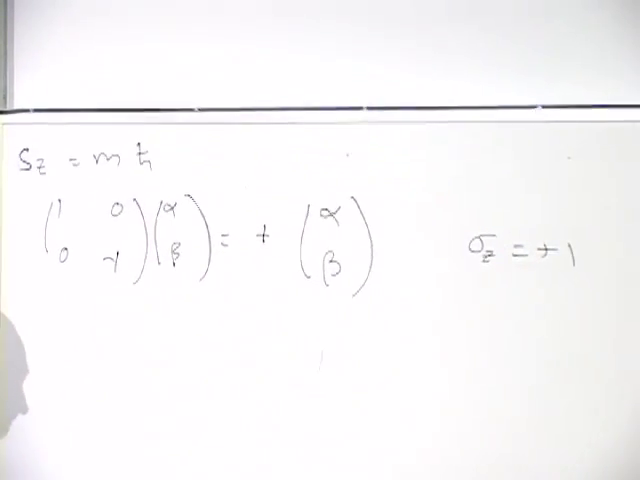
\includegraphics[width=0.74\textwidth]{lecture_08_figure_02.png}
\caption{二分量旋量在\(\sigma_z\)作用下滿足的\(+1\)本徵值方程。}
\lectureframe{00:34:57}
\end{figure}

對於本徵值\(+1\)，逐行相乘可得
\begin{equation}
\begin{pmatrix}
1\cdot\alpha+0\cdot\beta\\
0\cdot\alpha-\beta
\end{pmatrix}
=
\begin{pmatrix}
\alpha\\
-\beta
\end{pmatrix}
=
\begin{pmatrix}
\alpha\\
\beta
\end{pmatrix}.
\end{equation}
上方的方程自動成立；下方的方程則給出\(-\beta=\beta\)，所以\(\beta=0\)。歸一化條件要求\(|\alpha|=1\)；選擇任意的整體相位，使\(\alpha=1\)，便得到
\begin{equation}
|+z\rangle=
\begin{pmatrix}
1\\
0
\end{pmatrix}.
\end{equation}

對於本徵值\(-1\)，
\begin{equation}
\begin{pmatrix}
\alpha\\
-\beta
\end{pmatrix}
=
\begin{pmatrix}
-\alpha\\
-\beta
\end{pmatrix}.
\end{equation}
這時下方的方程自動成立，上方的方程給出\(\alpha=-\alpha\)，因此\(\alpha=0\)。令\(\beta=1\)，便得到
\begin{equation}
|-z\rangle=
\begin{pmatrix}
0\\
1
\end{pmatrix}.
\end{equation}

現在改為測量\(S_x\)。由於
\begin{equation}
\sigma_x
\begin{pmatrix}
\alpha\\
\beta
\end{pmatrix}
=
\begin{pmatrix}
0\cdot\alpha+\beta\\
\alpha+0\cdot\beta
\end{pmatrix}
=
\begin{pmatrix}
\beta\\
\alpha
\end{pmatrix},
\end{equation}
本徵值為\(+1\)的方程變成
\begin{equation}
\begin{pmatrix}
\beta\\
\alpha
\end{pmatrix}
=
\begin{pmatrix}
\alpha\\
\beta
\end{pmatrix}.
\end{equation}
兩個分量方程\(\beta=\alpha\)和\(\alpha=\beta\)表達的是同一個條件。歸一化後得到
\begin{equation}
2|\alpha|^2=1,
\end{equation}
因此，一個方便的選擇是
\begin{equation}
|+x\rangle
=
\frac{1}{\sqrt2}
\begin{pmatrix}
1\\
1
\end{pmatrix}.
\end{equation}

\begin{figure}[t]
\centering
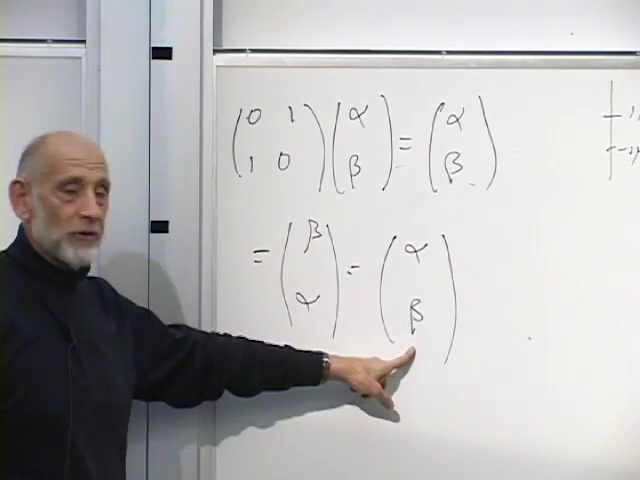
\includegraphics[width=0.74\textwidth]{lecture_08_figure_03.png}
\caption{本徵值為\(+1\)時，\(\sigma_x\)會交換兩個分量，因此必須滿足\(\alpha=\beta\)。}
\lectureframe{00:39:42}
\end{figure}

\begin{classroomqa}
\lecturetimestamp{00:40:13}
\audiencequestion{如果納入二分之一因子，本徵值會是二分之一嗎？}
\lecturerresponse{是的。泡利矩陣\(\sigma_x\)的本徵值是\(\pm1\)；而\(S_x=\sigma_x/2\)的本徵值是\(\pm\tfrac12\)。}
\end{classroomqa}

對於本徵值\(-1\)，
\begin{equation}
\begin{pmatrix}
\beta\\
\alpha
\end{pmatrix}
=
-
\begin{pmatrix}
\alpha\\
\beta
\end{pmatrix},
\end{equation}
所以
\begin{equation}
\beta=-\alpha,
\qquad
\alpha=-\beta.
\end{equation}
這兩個方程同樣表達相同條件。歸一化後，
\begin{equation}
|-x\rangle
=
\frac{1}{\sqrt2}
\begin{pmatrix}
1\\
-1
\end{pmatrix}.
\end{equation}
因此，\(z\)向上與\(z\)向下的等量疊加態，具有沿正\(x\)軸的極化；若兩者之間帶有相對負號，則具有沿負\(x\)軸的極化。

對於\(y\)方向，
\begin{equation}
\sigma_y
\begin{pmatrix}
\alpha\\
\beta
\end{pmatrix}
=
\begin{pmatrix}
-i\beta\\
i\alpha
\end{pmatrix}.
\end{equation}
兩個歸一化本徵向量為
\begin{equation}
|+y\rangle
=
\frac{1}{\sqrt2}
\begin{pmatrix}
1\\
i
\end{pmatrix},
\qquad
|-y\rangle
=
\frac{1}{\sqrt2}
\begin{pmatrix}
1\\
-i
\end{pmatrix},
\end{equation}
差別僅在整體相位。兩個態測得\(z\)向上的機率都是\(1/2\)，測得\(z\)向下的機率都是\(1/2\)。相對相位\(i\)不會顯現在這兩個機率中，卻能區分\(y\)極化和\(x\)極化。線性組合也可以描述沿任意方向極化的自旋，相關計算留待後續討論。

\begin{classroomqa}
\lecturetimestamp{00:44:22}
\audiencequestion{\(\sigma_y\)的\(i\)分量是否被配上了錯誤的本徵值？}
\lecturerresponse{這個符號的確可能配錯了本徵值。這裡無法確定正確的配法，因此不憑記憶下定論。}
\end{classroomqa}

直接計算可得
\begin{align}
\sigma_y\frac{1}{\sqrt2}
\begin{pmatrix}
1\\
i
\end{pmatrix}
&=
\frac{1}{\sqrt2}
\begin{pmatrix}
-i\,i\\
i
\end{pmatrix}
=
\frac{1}{\sqrt2}
\begin{pmatrix}
1\\
i
\end{pmatrix},\\
\sigma_y\frac{1}{\sqrt2}
\begin{pmatrix}
1\\
-i
\end{pmatrix}
&=
\frac{1}{\sqrt2}
\begin{pmatrix}
(-i)(-i)\\
i
\end{pmatrix}
=
-\frac{1}{\sqrt2}
\begin{pmatrix}
1\\
-i
\end{pmatrix}.
\end{align}
因此，\(+i\)對應本徵值\(+1\)；\(-i\)則對應本徵值\(-1\)。\footnote{口述時對應關係幾經反覆，仍未確定；此處的符號則以所示矩陣乘法的結果為準。}每個自旋二分之一態，包括沿任意方向極化的態，都是\(|+z\rangle\)和\(|-z\rangle\)的線性組合。

\section{自旋一與位置依賴的旋量}

對於自旋\(1\)，\(S_z\)的可能值為\(+1,0,-1\)，因此態空間是三維的。自旋\(1\)是整數自旋，對應玻色統計。我們要找出三個滿足相同角動量對易關係的\(3\times3\)矩陣。

以下給出一種對三個座標方向一視同仁的表示法。\footnote{\(S_y\)的符號依據\(00{:}48{:}50\)附近顯示的矩陣，也由\([S_x,S_y]=iS_z\)確定。若將這個符號反轉，所需的對易關係也會跟著反轉。}
\begin{equation}
\begin{aligned}
S_x
&=
i
\begin{pmatrix}
0&0&0\\
0&0&1\\
0&-1&0
\end{pmatrix},
&
S_y
&=
i
\begin{pmatrix}
0&0&1\\
0&0&0\\
-1&0&0
\end{pmatrix},\\
S_z
&=
i
\begin{pmatrix}
0&1&0\\
-1&0&0\\
0&0&0
\end{pmatrix}.
\end{aligned}
\end{equation}
每個矩陣都是\(i\)乘上一個實反對稱矩陣。每個矩陣各含有一個\(1\)、一個\(-1\)，並且與自身座標相對應的行和列皆為零：第一個對應\(S_x\)，第二個對應\(S_y\)，第三個對應\(S_z\)。這可以當作一個好記的口訣。在這種表示法中，\(S_z\)不是對角矩陣。

令
\begin{equation}
v=
\begin{pmatrix}
\alpha\\
\beta\\
\gamma
\end{pmatrix}.
\end{equation}
則
\begin{equation}
S_zv
=
\begin{pmatrix}
i\beta\\
-i\alpha\\
0
\end{pmatrix}.
\end{equation}
對於本徵值\(+1\)，
\begin{equation}
i\beta=\alpha,
\qquad
-i\alpha=\beta,
\qquad
0=\gamma.
\end{equation}
因此\(\beta=-i\alpha\)，且\(\gamma=0\)。歸一化條件給出\(2|\alpha|^2=1\)，所以
\begin{equation}
|m=+1\rangle
=
\frac{1}{\sqrt2}
\begin{pmatrix}
1\\
-i\\
0
\end{pmatrix}.
\end{equation}
對於本徵值\(-1\)，
\begin{equation}
i\beta=-\alpha,
\qquad
-i\alpha=-\beta,
\qquad
0=-\gamma,
\end{equation}
因此\(\beta=i\alpha\)、\(\gamma=0\)，並得到
\begin{equation}
|m=-1\rangle
=
\frac{1}{\sqrt2}
\begin{pmatrix}
1\\
i\\
0
\end{pmatrix}.
\end{equation}
最後，零本徵值方程給出\(\alpha=\beta=0\)，而\(\gamma\)仍可任意取值。歸一化後的解為
\begin{equation}
|m=0\rangle
=
\begin{pmatrix}
0\\
0\\
1
\end{pmatrix}.
\end{equation}
這三個本徵向量已經涵蓋整個三維空間，不存在其他本徵值。因子\(1/\sqrt2\)並非無關緊要；之後將這套代數應用於同位旋時，相同係數會出現在定量的實驗預測中。

\begin{classroomqa}
\lecturetimestamp{00:54:10}
\audiencequestion{這些自旋一本徵向量中的複數分量應該如何解讀？}
\lecturerresponse{當\(m=+1\)時，分量為\(1/\sqrt2,-i/\sqrt2,0\)；當\(m=-1\)時，分量為\(1/\sqrt2,i/\sqrt2,0\)；而當\(m=0\)時，分量為\(0,0,1\)。}
\end{classroomqa}

其他矩陣三元組也滿足相同的代數，且在物理上等價。上述對稱表示法的優點是平等看待三個方向，而且後面還會再用到它。

\subsection{恢復位置自由度}

現在把粒子的運動納入考量。自旋與位置、動量都對易，因此可以同時指定位置或動量以及一個自旋分量。位置與動量彼此不對易，不同的自旋分量之間也不對易。

運動中的自旋二分之一粒子以位置依賴的旋量描述：
\begin{equation}
\psi(x)=
\begin{pmatrix}
\psi_\uparrow(x)\\
\psi_\downarrow(x)
\end{pmatrix}.
\end{equation}
以下各量
\begin{equation}
\rho_{\uparrow_z}(x)=|\psi_\uparrow(x)|^2,
\qquad
\rho_{\downarrow_z}(x)=|\psi_\downarrow(x)|^2
\end{equation}
是位置與自旋的聯合機率密度。將它們相加，
\begin{equation}
\rho(x)=\psi^\dagger(x)\psi(x)
=|\psi_\uparrow(x)|^2+|\psi_\downarrow(x)|^2,
\end{equation}
便得到位置密度。若已知粒子在\(x\)處被偵測到，條件機率為
\begin{equation}
P(\uparrow_z\mid x)
=
\frac{|\psi_\uparrow(x)|^2}{\psi^\dagger(x)\psi(x)},
\qquad
P(\downarrow_z\mid x)
=
\frac{|\psi_\downarrow(x)|^2}{\psi^\dagger(x)\psi(x)},
\end{equation}
只要\(\rho(x)\neq0\)。因此，電子由一個二分量的空間波函數描述，局部的自旋振幅可以隨位置而變化。

運動中的自旋一粒子可寫成
\begin{equation}
\phi(x)=
\begin{pmatrix}
\phi_1(x)\\
\phi_2(x)\\
\phi_3(x)
\end{pmatrix}.
\end{equation}
在空間中的每一點，三個分量都構成上述同一自旋空間中的一個向量。自旋一粒子具有整數自旋，因此是玻色子。

\begin{classroomqa}
\lecturetimestamp{01:00:10}
\audiencequestion{\(\phi_1(x)\)本身就是自旋一的\(m=+1\)結果機率嗎？}
\lecturerresponse{不是。它是在所選三分量基底中的振幅。若要得到確定的自旋測量結果，先取相應歸一化本徵向量的左矢，將場投影到該左矢上，再取模平方。}
\end{classroomqa}

\begin{figure}[t]
\centering
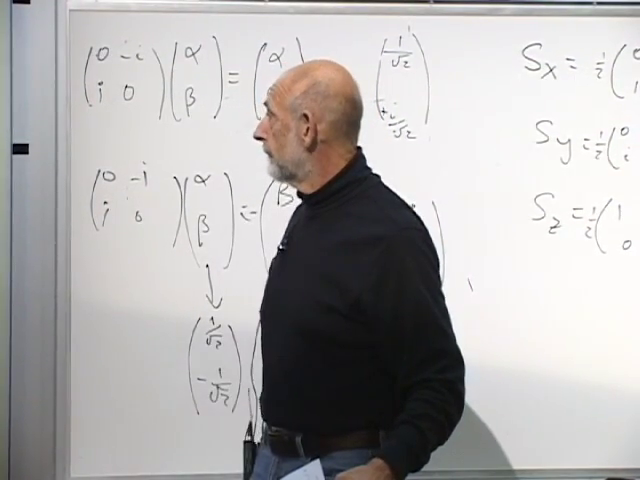
\includegraphics[width=0.82\textwidth]{lecture_08_figure_04.png}
\caption{歸一化的\(\sigma_y\)本徵向量，與三個自旋二分之一矩陣並列。}
\lectureframe{01:00:12}
\end{figure}

例如，
\begin{equation}
\begin{aligned}
|m=+1\rangle
&=
\frac{1}{\sqrt2}
\begin{pmatrix}
1\\
-i\\
0
\end{pmatrix}
\\
\Longrightarrow\quad\langle m=+1|
&=
\frac{1}{\sqrt2}
\begin{pmatrix}
1&i&0
\end{pmatrix}.
\end{aligned}
\end{equation}
因此，投影振幅為
\begin{align}
\langle m=+1|\phi(x)\rangle
&=
\frac{1}{\sqrt2}
\begin{pmatrix}
1&i&0
\end{pmatrix}
\begin{pmatrix}
\phi_1(x)\\
\phi_2(x)\\
\phi_3(x)
\end{pmatrix}\\
&=
\frac{\phi_1(x)+i\phi_2(x)}{\sqrt2}.
\end{align}
對三個本徵向量都套用相同規則，就能得到各自旋分量的密度。\footnote{明確修正\(\phi_1\)和\(\phi_2\)不一定是實數後，這些公式便完整描述了投影代數。若把它們當作實數，就會錯誤地消去區分\(m=+1\)與\(m=-1\)密度的干涉效應。}
\begin{align}
\rho_{+1}(x)
&=
\frac12\left|\phi_1(x)+i\phi_2(x)\right|^2,\\
\rho_{-1}(x)
&=
\frac12\left|\phi_1(x)-i\phi_2(x)\right|^2,\\
\rho_0(x)
&=
|\phi_3(x)|^2.
\end{align}
它們滿足
\begin{equation}
\begin{aligned}
\rho_{+1}(x)+\rho_{-1}(x)+\rho_0(x)
&=
|\phi_1(x)|^2+|\phi_2(x)|^2
\\
&\quad{}+|\phi_3(x)|^2
\\
&=
\phi^\dagger(x)\phi(x).
\end{aligned}
\end{equation}
若已知粒子在\(x\)處被偵測到，則
\begin{equation}
P(m\mid x)
=
\frac{\rho_m(x)}{\phi^\dagger(x)\phi(x)},
\end{equation}
只要\(\phi^\dagger(x)\phi(x)\neq0\)。一般的測量規則始終相同：取出目標歸一化本徵向量的左矢，將實際態投影到它上面，再取模平方。所得密度仍保留對位置的依賴。

更高自旋的矩陣較為複雜，但原理不變。

\begin{classroomqa}
\lecturetimestamp{01:07:31}
\audiencequestion{自旋三分之二的態空間有多大？}
\lecturerresponse{共有四個態，其中\(m=\tfrac32,\tfrac12,-\tfrac12,-\tfrac32\)。自旋二則有五個態。}
\end{classroomqa}

\begin{classroomqa}
\lecturetimestamp{01:07:55}
\audiencequestion{為什麼討論中出現了\(x,y,z\)，卻沒有時間方向？這套處理是非相對論性的嗎？}
\lecturerresponse{到目前為止，這套處理是非相對論性的。自旋和質量一樣，在粒子的靜止系中最容易描述；在其他慣性系中的描述，則由相應的洛倫茲變換得到。這個相對論性的步驟留待後續討論。}
\end{classroomqa}

狄拉克方程提供了相對論性的框架，也說明為什麼它的四分量波函數包含一個自旋雙重態。

\section{狄拉克矩陣與四分量旋量}

四分量狄拉克波函數滿足
\begin{equation}
i\frac{\partial\Psi}{\partial t}
=
-i\alpha_i\frac{\partial\Psi}{\partial x_i}
+m\beta\Psi,
\qquad i=1,2,3,
\end{equation}
其中重複的空間指標代表求和。因此，導數項就是
\begin{equation}
\alpha_1\frac{\partial\Psi}{\partial x}
+\alpha_2\frac{\partial\Psi}{\partial y}
+\alpha_3\frac{\partial\Psi}{\partial z}.
\end{equation}
對平面波而言，方程可化為代數形式
\begin{equation}
\omega\Psi=(\alpha_i k_i+m\beta)\Psi.
\end{equation}

\begin{classroomqa}
\lecturetimestamp{01:11:32}
\audiencequestion{兩處的\(m\)指的是同一件事嗎？}
\lecturerresponse{不是。一處將它用作空間指標，另一處則表示粒子的質量。將空間指標改記為\(i\)；當\(i\)出現兩次時，就要從\(1\)加到\(3\)求和。}
\end{classroomqa}

將頻率算符平方後，必須得到相對論關係式
\begin{equation}
\omega^2=\mathbf{k}^2+m^2.
\end{equation}
因此，對每個\(i\)，平方項都必須滿足
\begin{equation}
\alpha_i^2=I_4,
\qquad
\beta^2=I_4.
\end{equation}

\begin{classroomqa}
\lecturetimestamp{01:13:01}
\audiencequestion{\(\beta\)在\(\Psi\)的四個分量中各不相同嗎？}
\lecturerresponse{不是。只有一個矩陣\(\beta\)作用於整個四分量旋量，而且它滿足\(\beta^2=I_4\)。}
\end{classroomqa}

混合項必須消失。不同空間方向的矩陣彼此之間，以及每個\(\alpha_i\)與\(\beta\)之間，都必須滿足
\begin{equation}
\alpha_i\alpha_j+\alpha_j\alpha_i=0
\quad (i\neq j),
\qquad
\alpha_i\beta+\beta\alpha_i=0.
\end{equation}
等價地，
\begin{equation}
\{\alpha_i,\alpha_j\}=2\delta_{ij}I_4,
\quad
\{\alpha_i,\beta\}=0,
\quad
\{\beta,\beta\}=2I_4.
\end{equation}
每個矩陣都與其他不同的矩陣反對易；矩陣與自身的反對易子則等於單位矩陣的兩倍。

若沒有\(\beta\)，三個泡利矩陣已經提供了三個平方等於單位矩陣、且兩兩反對易的\(2\times2\)矩陣。質量項還要求第四個具有相同性質的矩陣。不存在符合這些條件的第四個\(2\times2\)矩陣，而\(3\times3\)矩陣也無法滿足這套代數。因此，最小表示的維度是\(4\times4\)。

一個\(4\times4\)矩陣可以分成四個\(2\times2\)區塊。在一種方便的表示法中，
\begin{equation}
\alpha_i=
\begin{pmatrix}
\sigma_i&0\\
0&-\sigma_i
\end{pmatrix},
\qquad i=1,2,3.
\end{equation}

\begin{figure}[t]
\centering
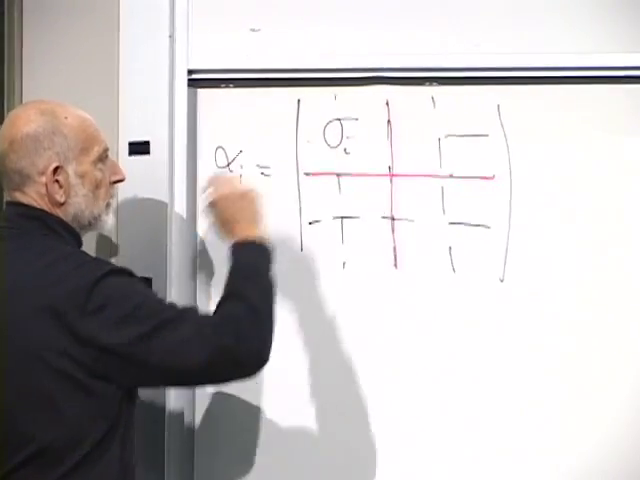
\includegraphics[width=0.68\textwidth]{lecture_08_figure_05.png}
\caption{狄拉克矩陣\(\alpha_i\)以\(2\times2\)區塊表示，\(\sigma_i\)和\(-\sigma_i\)位於對角線上。}
\lectureframe{01:17:23}
\end{figure}

\begin{classroomqa}
\lecturetimestamp{01:17:41}
\audiencequestion{早先的表示法中，\(\sigma_i\)區塊是不是以相反的方式排列？}
\lecturerresponse{是的。另一種表示法把它們放在非對角線位置。這兩種排列彼此等價，並由相似變換連結。}
\end{classroomqa}

在目前的表示法中，另一個矩陣是
\begin{equation}
\beta=
\begin{pmatrix}
0&I_2\\
I_2&0
\end{pmatrix},
\qquad
I_2=
\begin{pmatrix}
1&0\\
0&1
\end{pmatrix}.
\end{equation}
透過區塊矩陣乘法，只需進行一般\(2\times2\)矩陣的乘法，就能檢驗\(4\times4\)代數。

\begin{classroomqa}
\lecturetimestamp{01:19:17}
\audiencequestion{早先的表示法中，\(\beta\)是不是具有不同的符號或對角形式？}
\lecturerresponse{早先採用的是不同但在物理上等價的基底。基底變換會混合\(\Psi\)的四個分量，改變矩陣的形式，但不改變物理。}
\end{classroomqa}

\(\Psi\)的四個分量不是時空的四個座標，而是這套反對易代數能作用的最小向量空間中的座標。這裡有兩種不同的二重結構：分成\(2\times2\)區塊的結構，以及每個區塊內部的二分量泡利結構。先看下文將建立的詮釋，四種可能性可以整理如下：
\begin{equation}
\begin{array}{c|cc}
& S_z=+\tfrac12 & S_z=-\tfrac12\\ \hline
\omega>0 & (\omega>0,+\tfrac12) & (\omega>0,-\tfrac12)\\
\omega<0 & (\omega<0,+\tfrac12) & (\omega<0,-\tfrac12)
\end{array}.
\end{equation}
下一列代表負頻率的電子態，不是正電子。正電子將被詮釋為這組態全部填滿後所留下的一個電洞。

\section{靜止系能量的倍增與正電子}

在零動量處，最容易看出能量的二重結構。當\(\mathbf{k}=0\)時，平面波態在空間中為常數，空間導數項也就消失。靜止系方程\footnote{在\(01{:}23{:}38\)的畫面中，質量項暫時多出了一個因子\(i\)；\(01{:}24{:}05\)處的口頭更正則將它去除。}為
\begin{equation}
i\frac{\partial\Psi}{\partial t}=m\beta\Psi.
\end{equation}

\begin{figure}[t]
\centering
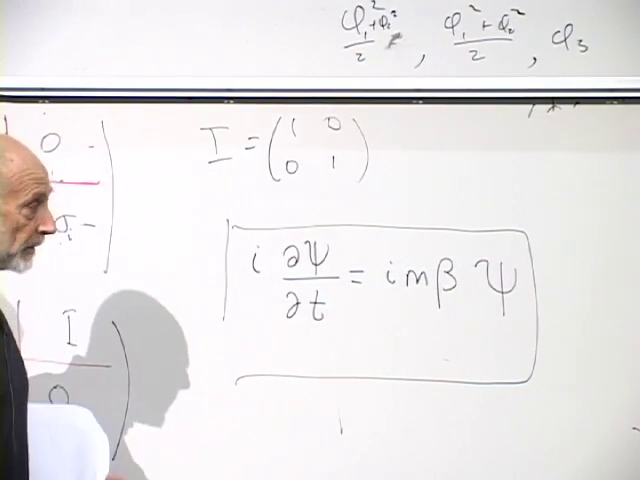
\includegraphics[width=0.76\textwidth]{lecture_08_figure_06.png}
\caption{零動量時空間導數消失，剩下修正後的靜止系方程\(i\partial_t\Psi=m\beta\Psi\)。}
\lectureframe{01:23:38}
\end{figure}

將四分量直欄向量分成上、下兩個二分量向量：
\begin{equation}
\Psi=
\begin{pmatrix}
\psi_+\\
\psi_-
\end{pmatrix}.
\end{equation}

\begin{classroomqa}
\lecturetimestamp{01:24:47}
\audiencequestion{標記 \(\psi_+\) 和 \(\psi_-\) 已經代表正能量和負能量了嗎？}
\lecturerresponse{還沒有。在這個階段，它們只是上、下兩個二分量區塊的名稱，還沒有求出它們對應的能量組合。}
\end{classroomqa}

\begin{classroomqa}
\lecturetimestamp{01:25:10}
\audiencequestion{分成兩部分的四分量列向量代表什麼？}
\lecturerresponse{它仍是同一個四分量狄拉克旋量，只是按照矩陣的區塊形式重新排列。每一半都是二分量物件，兩個這樣的物件合起來就是原本的四分量列向量。}
\end{classroomqa}

矩陣 \(\beta\) 會交換這兩個區塊：
\begin{equation}
\beta
\begin{pmatrix}
\psi_+\\
\psi_-
\end{pmatrix}
=
\begin{pmatrix}
\psi_-\\
\psi_+
\end{pmatrix}.
\end{equation}
因此，靜止系中的方程變為
\begin{equation}
i\frac{\partial\psi_+}{\partial t}=m\psi_-,
\qquad
i\frac{\partial\psi_-}{\partial t}=m\psi_+.
\end{equation}

有兩種自然的做法。再取一次時間導數可以將系統解耦；不過，將兩個方程相加與相減，就能立即將它們對角化。具體而言，
\begin{align}
i\frac{\partial}{\partial t}(\psi_++\psi_-)
&=m(\psi_++\psi_-),\\
i\frac{\partial}{\partial t}(\psi_+-\psi_-)
&=-m(\psi_+-\psi_-).
\end{align}
定義
\begin{equation}
\chi_+=\psi_++\psi_-,
\qquad
\chi_-=\psi_+-\psi_-,
\end{equation}
便得到兩個互相獨立的方程：
\begin{equation}
i\partial_t\chi_+=m\chi_+,
\qquad
i\partial_t\chi_-=-m\chi_-.
\end{equation}
若時間依賴具有確定頻率 \(e^{-i\omega t}\)，和所對應的頻率為
\begin{equation}
\omega=+m,
\end{equation}
差所對應的頻率則為
\begin{equation}
\omega=-m.
\end{equation}
這正是先前一維例子中出現的正、負能量雙重結構：相對論方程再次具有正能量與負能量的電子解。因此，區塊的雙重結構分解為正能量與負能量兩個分支。純粹的靜止態可以寫成
\begin{equation}
\Psi_{\omega=+m}=
\begin{pmatrix}
\xi\\
\xi
\end{pmatrix},
\qquad
\Psi_{\omega=-m}=
\begin{pmatrix}
\xi\\
-\xi
\end{pmatrix},
\end{equation}
其中 \(\xi\) 仍是任意的二分量物件。

相加與相減已經分解了一種雙重結構，但 \(\xi\) 的兩個分量仍然存在。泡利矩陣作用於這一對剩餘分量。這一對與自旋相關；不過，還必須通過下文所述的旋轉或守恆定律檢驗，才能確認這一點。

\begin{classroomqa}
\lecturetimestamp{01:32:23}
\audiencequestion{可以把自旋看作外層的雙重結構，把能量正負看作內層的雙重結構嗎？}
\lecturerresponse{可以。這兩種因子的排列順序彼此等價，可以交換哪個指標寫在前面；這只會重新排列四個分量。}
\end{classroomqa}

負頻率分支引出了狄拉克海的詮釋。負頻率被賦予負的電子能量。將所有負能量電子態填滿，便能在泡利不相容原理允許的範圍內，盡可能降低能量，因為每個完整的費米子態只能容納一個電子。完全填滿的負能量海於是稱為真空。

將這個填滿的海中的一個電子提升到正能量態。結果會有一個正能量電子，以及一個未被佔據的負能量態。移去一個負能量會使能量升高，因此這個空穴具有正的激發能；由於少了一個電子，它也帶有與電子相反的電荷。這個空穴就是正電子。

\begin{classroomqa}
\lecturetimestamp{01:32:57}
\audiencequestion{可以再說明一次正電子的詮釋嗎？}
\lecturerresponse{兩個區塊相加得到正頻率，兩者相減則得到負頻率。負頻率解是負能量電子態；真空則是將這些態全部填滿後的狀態。把一個已填入的電子提升到正能量後，便同時留下正能量電子和一個空穴。這個具有正能量、帶相反電荷的空穴就是正電子。}
\end{classroomqa}

因此，這套代數同時帶來兩項結果：正能量與負能量分支，形成粒子--反粒子結構；以及與自旋二分之一相關的剩餘二分量結構。引人注目的是，這兩者都來自能夠滿足相對論性反對易關係的最小矩陣。當時，自旋才剛被發現是一種經驗性質；在這樣的歷史背景下，這套數學構造竟然導出具有自旋的粒子以及反粒子分支，結果十分驚人。

\begin{classroomqa}
\lecturetimestamp{01:35:14}
\audiencequestion{負能量電子本身就是正電子嗎？}
\lecturerresponse{不是。真空中的負能量電子態都已填滿。正電子是這些已填滿的態中少了一個電子，也就是一個空穴，而不是負能量電子。}
\end{classroomqa}

空穴也可以參與躍遷。正電子具有正能量，是因為它代表少了一個負能量電子。如果一個正能量電子填入空穴，電子與正電子便會湮滅，但能量必須由其他東西帶走，通常是光子。用狄拉克海的說法，就是一個電子填入原本未被佔據的負能量態。同樣的能量釋放，也可以想成原子中的激發態電子降至較低能階：電子向下躍遷時會放出光子。

\begin{classroomqa}
\lecturetimestamp{01:36:39}
\audiencequestion{為什麼能量較高的負能量電子不會落入空穴？}
\lecturerresponse{這個問題混淆了兩種情況。正能量電子填入空穴，屬於電子--正電子湮滅，能量由光子帶走。負能量海中的電子發生躍遷則是另一種過程，下面會再討論。}
\end{classroomqa}

零動量的計算本身已經表明，分離出能量正負後，仍有二重簡併。但兩個態的簡併本身，並不能證明它們具有角動量。

\begin{classroomqa}
\lecturetimestamp{01:37:44}
\audiencequestion{零動量計算如何證明剩下的兩個態代表自旋？}
\lecturerresponse{可以把這兩個態稱為自旋向上和自旋向下；完整方程中也會出現泡利矩陣，但這些都還不足以構成證明。必須證明這一對態在空間旋轉下如何變換，或者證明賦予它們自旋後，總角動量在交互作用和碰撞中守恆。這項論證留待後續討論。}
\end{classroomqa}

對於正能量的靜止態，上、下兩個區塊相等：
\begin{equation}
\Psi_{\omega=+m}=
\begin{pmatrix}
\xi\\
\xi
\end{pmatrix}.
\end{equation}
要確立 \(\xi\) 構成角動量二重態，仍需要前述的旋轉論證或守恆論證；光是數出兩個分量，並不能得出這個結論。

\begin{classroomqa}
\lecturetimestamp{01:40:46}
\audiencequestion{即使能量不同，另一個電子也能和這個正電子湮滅嗎？}
\lecturerresponse{可以。電子沒有各自獨立的身分，任何可用的電子都可以填入空穴。初始能量與動量的差異，會反映在放出光子的數量與能量上。}
\end{classroomqa}

空穴圖像也能解釋完全發生在負能量海內部的躍遷。假設一個已佔據的負能量態移入空穴，原來的空穴便被填滿，但該電子原先所在的態現在空了。於是空穴移動了。換句話說，正電子改變了能量並放出輻射。

\begin{classroomqa}
\lecturetimestamp{01:42:12}
\audiencequestion{為什麼相鄰的負能量能階不能接連落入空穴？}
\lecturerresponse{它們可以使空穴從一個能階移到另一個能階。電子落入原來的空穴後，會在它原先的能量處留下新空穴，因此原本的正電子就變成能量不同的正電子。能量差由光子帶走。}
\end{classroomqa}

\begin{classroomqa}
\lecturetimestamp{01:44:39}
\audiencequestion{為什麼這不會造成無止盡的向下輻射級聯？}
\lecturerresponse{因為能量和動量必須同時守恆，這兩項守恆定律不允許這種不受限制的過程。普通的自由電子也有同樣的限制：它不能只靠在空無一物的空間中放出光子，就不斷降低能量。}
\end{classroomqa}
